% \subsection{Missing Information}

A shuffled deck of cards. A gas of who-knows-what. A messy room. When we say that these are high-entropy systems, we really mean that we lack the information needed to have a complete description. If a room is messy, how can one find a certain book? We do not know where it is. We know what the room looks \emph{like} but we cannot say much about the details. Conversely, in a tidy room, the book can easily be found because we are able, in our mind, to completely describe the room. A tidy room is a low-entropy system.

The physicist can approach entropy with a myriad of tools. The first is painting. Consider “The Disintegration of the Persistence of Memory” by Salvador Dali (Figure \ref{fig.painting}). Time is warped. Geometric structures turn about as if they are unsure which laws to follow. A discombobulated fish—is it alive or dead? or both simultaneously?—drowns in the ocean. The ocean drowns the land. Objects are reflected unnaturally, incompletely. The painting begs to be understood, but understanding is lacking. The closer you look, the more you realize that something is missing. It is as if we have lost a framework of knowledge. We have bits and pieces of memory but not the structure to understand all.

This is precisely what entropy is in physics. To say there is lots of entropy is to say much more information would be needed to understand every detail of reality. An increase in entropy is indeed a disintegration of the persistence of memory.

Having exhausted her patience for painting, the hasty physicist will now want equations. The first one defines the Gibbs entropy
\begin{equation}\label{eq.Gibbs_entropy_definition}
S = -\sum_{i=1}^N P_i \log P_i
\end{equation}
for a situation with \(N\) possibilities, each with probability \(P_i\). If \(N=1\), the entropy is zero and we say that the system is in a ``pure state.''  If \(N > 1\), the entropy is nonzero and we say that the system is in a ``mixed state.’’

In quantum mechanics, we can keep the exact same definition and merely clarify that by a \emph{possibility} we mean a \emph{possible wavefunction}. Then we call (\ref{eq.Gibbs_entropy_definition}) the Von Neumann entropy. It turns out that Von Neumann entropy is the only reasonable definition of entropy in quantum mechanics that properly corresponds to Gibbs entropy. \cite{heusler,bracken,donald}

Because we consider systems with multiple possible wavefunctions, we describe states with density operators, defined as
\[
\op{\rho} = \sum_i P_i \ket{\Psi_i}\bra{\Psi_i}
\]
where \(\{\ket{\Psi_i}\}\) are the possible wavefunctions and each has probability \(P_i\) of being the true wavefunction. By studying how the eigenvalues and eigenstates of the density operator change over time, we understand how the probabilities and states change over time.

We can now write the Von Neumann entropy as a trace: \(S = -\Tr{\op{\rho} \log \op{\rho}}\).

\subsection{The subsystem entropy}

If we have a bipartite system \(\hilb_A \otimes \hilb_B\) and a basis \(\{\ket{\beta_m}\}\) for \(\hilb_B\), we can define the reduced density operator
\[
\overline{\op{\rho}} = \sum_m \left(\cdot \otimes \bra{\beta_m}\right) \op{\rho} \left(\cdot \otimes \ket{\beta_m}\right)
\]
that acts on the space \(\hilb_A\). Then the \(\hilb_A\)-subsystem entropy is \(-\Tr{\overline{\op{\rho}}\log \overline{\op{\rho}}}\).

We can think of \(\overline{\op{\rho}}\) as a version of \(\op{\rho}\) that is ``averaged out’’ at the resolution of \(\hilb_A\). We can gain insight with some probability theory. If we consider \(\op{\rho}\) to be a random variable, measurable on the sigma-algebra \(\hilb_A \otimes \hilb_B\), and we understand \(\hilb_A\) to be sub-sigma-algebra of \(\hilb_A \otimes \hilb_B\), then we can identify \(\overline{\op{\rho}}\) with the conditional expectation \(\ex \op{\rho} \,| \hilb_A\). In this sense, the subsystem entropy describes how much information is lost when we average out (take the conditional expectation).

(A sigma-algebra is a kind of algebraic structure at the centre of measure theory and probability theory. The probability-theory interpretation that I allude to here requires a bit more work to make precise---for example, Hilbert spaces correspond to sigma-algebras but are not sigma-algebras \emph{per se}.)

But how does subsystem entropy arise, and why is it useful? Let us consider the example of the double slit experiment.

\subsection{Example: the double slit experiment}\label{sec.doubleslit}

A particle is launched towards two slits, passes through the slits, lands on a detector, and has its position measured. Quantum mechanics predicts (and experiments verify) that the particle’s wavefunction will pass through \emph{both} slits simultaneously. The wavefunction through the upper slit will interfere with the wavefunction through the lower slit, creating a beautiful fringe pattern in the distribution of positions (Figure \ref{fig.quantum}).

\begin{figure}[bt]
\begin{subfigure}[t]{0.48\textwidth}
    \centering
    \begin{framed}
    \centering
    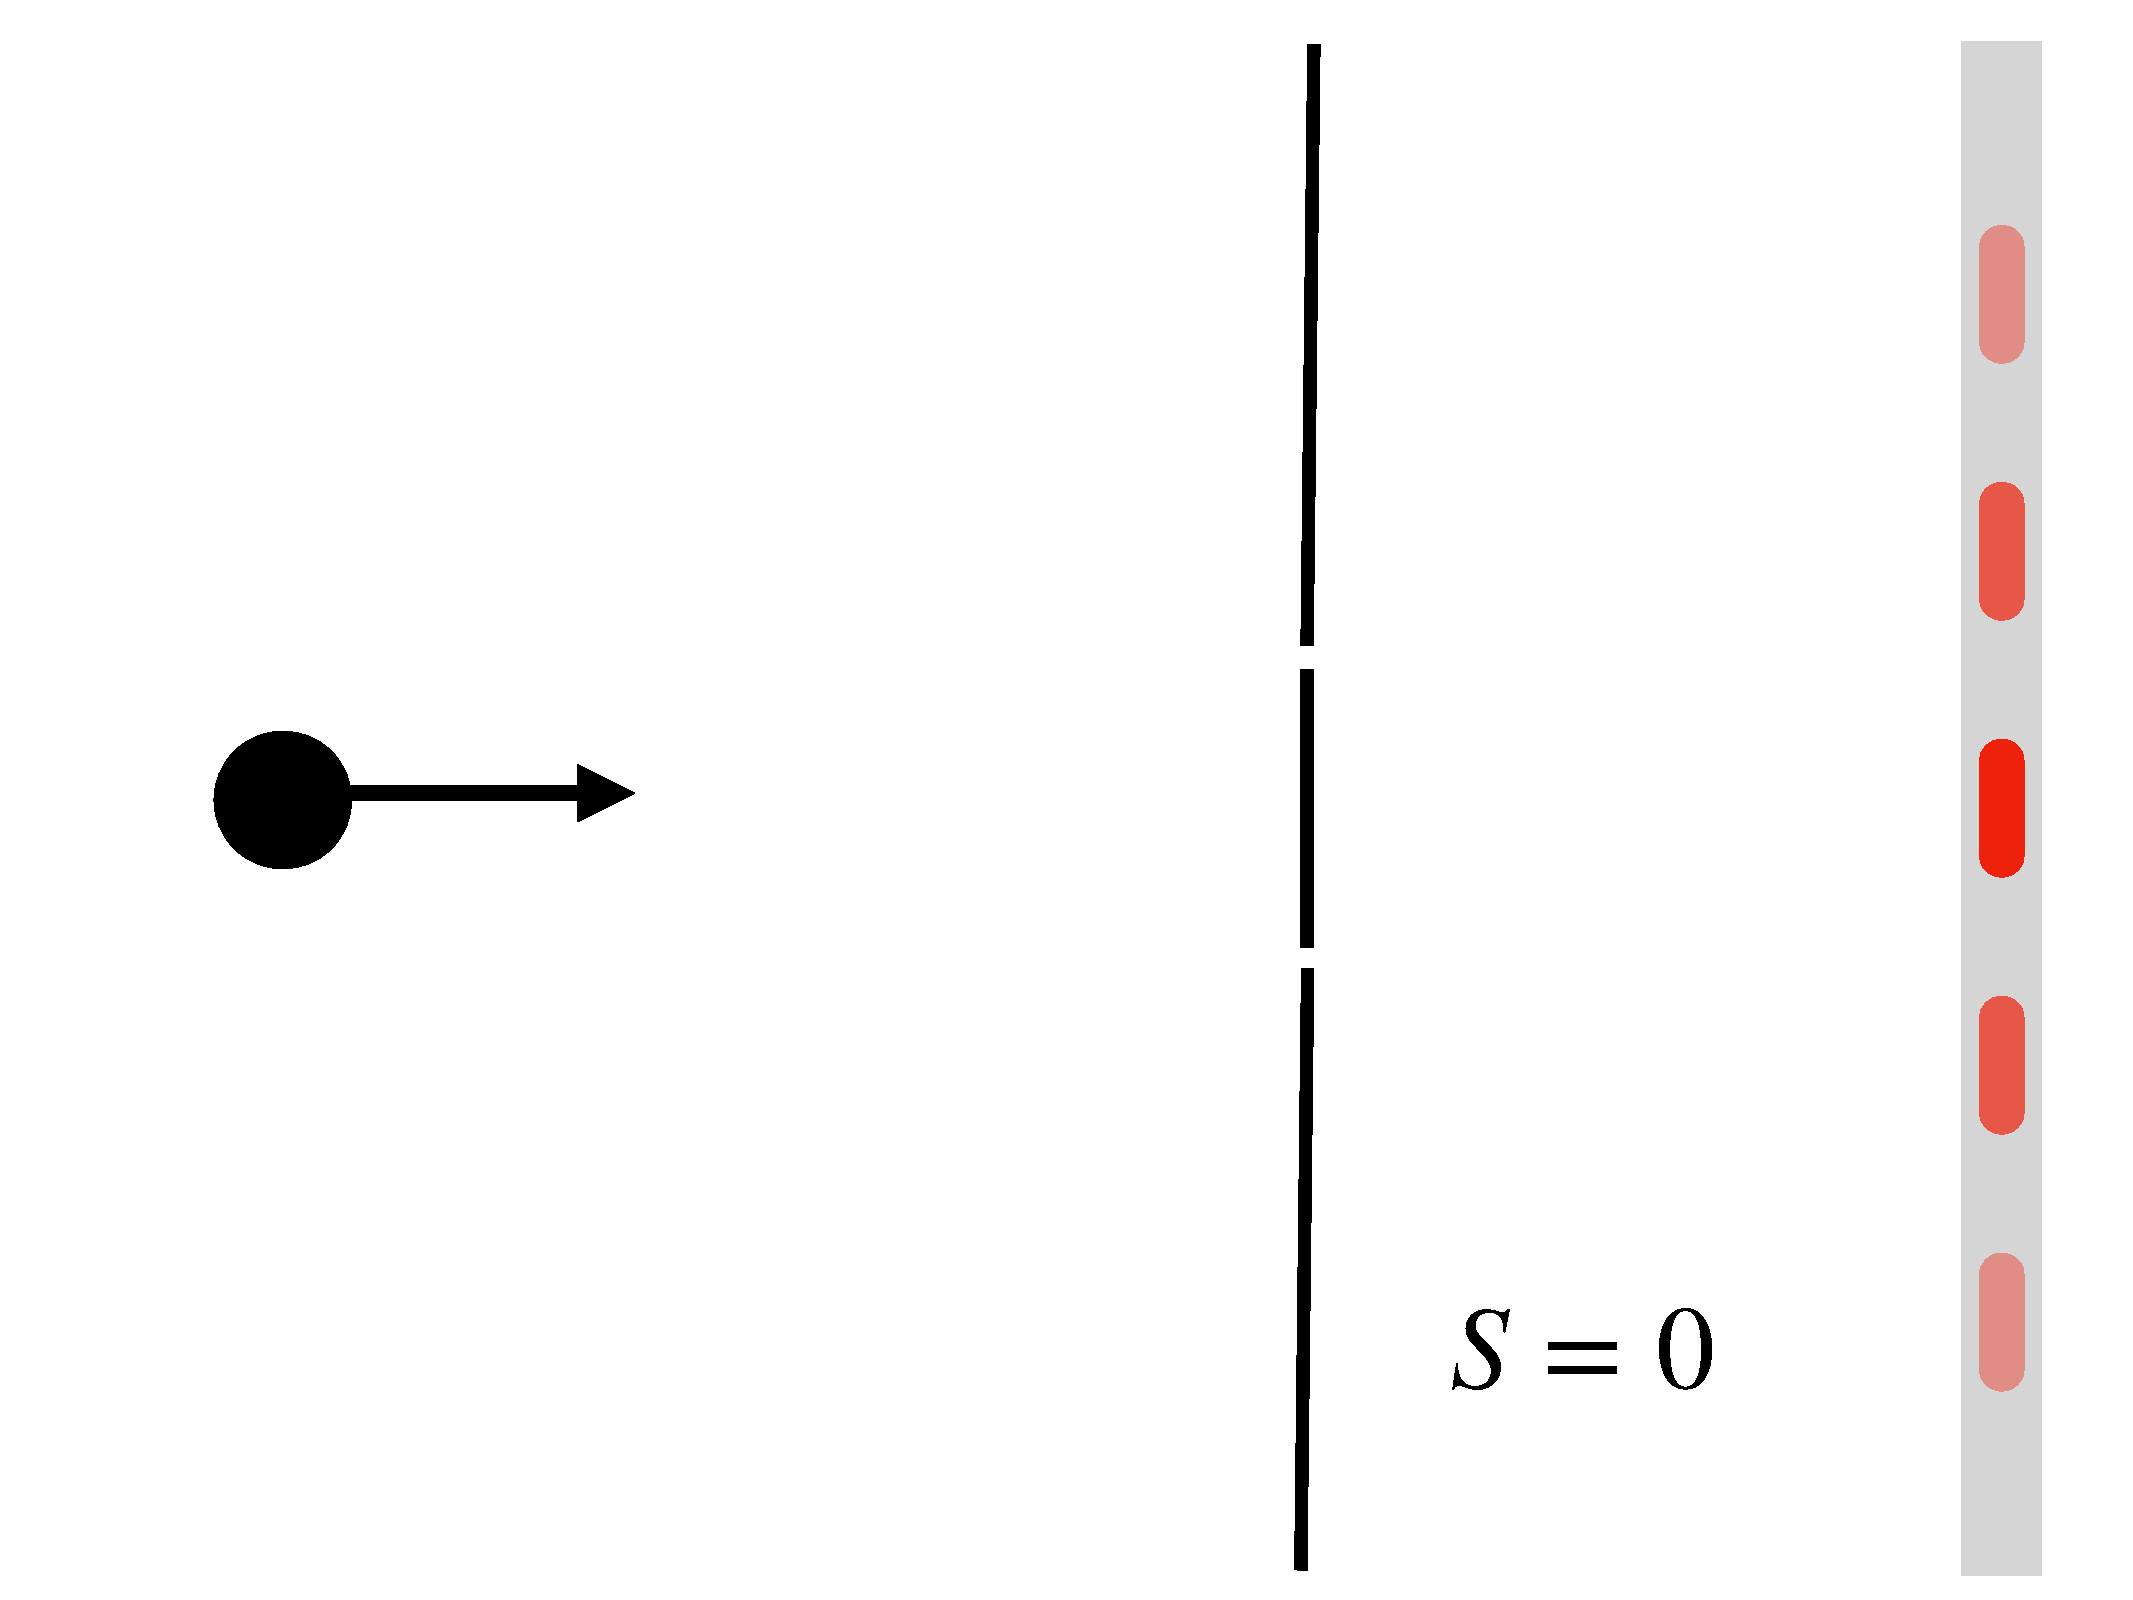
\includegraphics[width=\linewidth]{Figures/quantum}
    \caption{Quantum behaviour}
    \label{fig.quantum}
    \end{framed}
\end{subfigure}
\hfill
\begin{subfigure}[t]{0.48\textwidth}
    \centering
    \begin{framed}
    \centering
    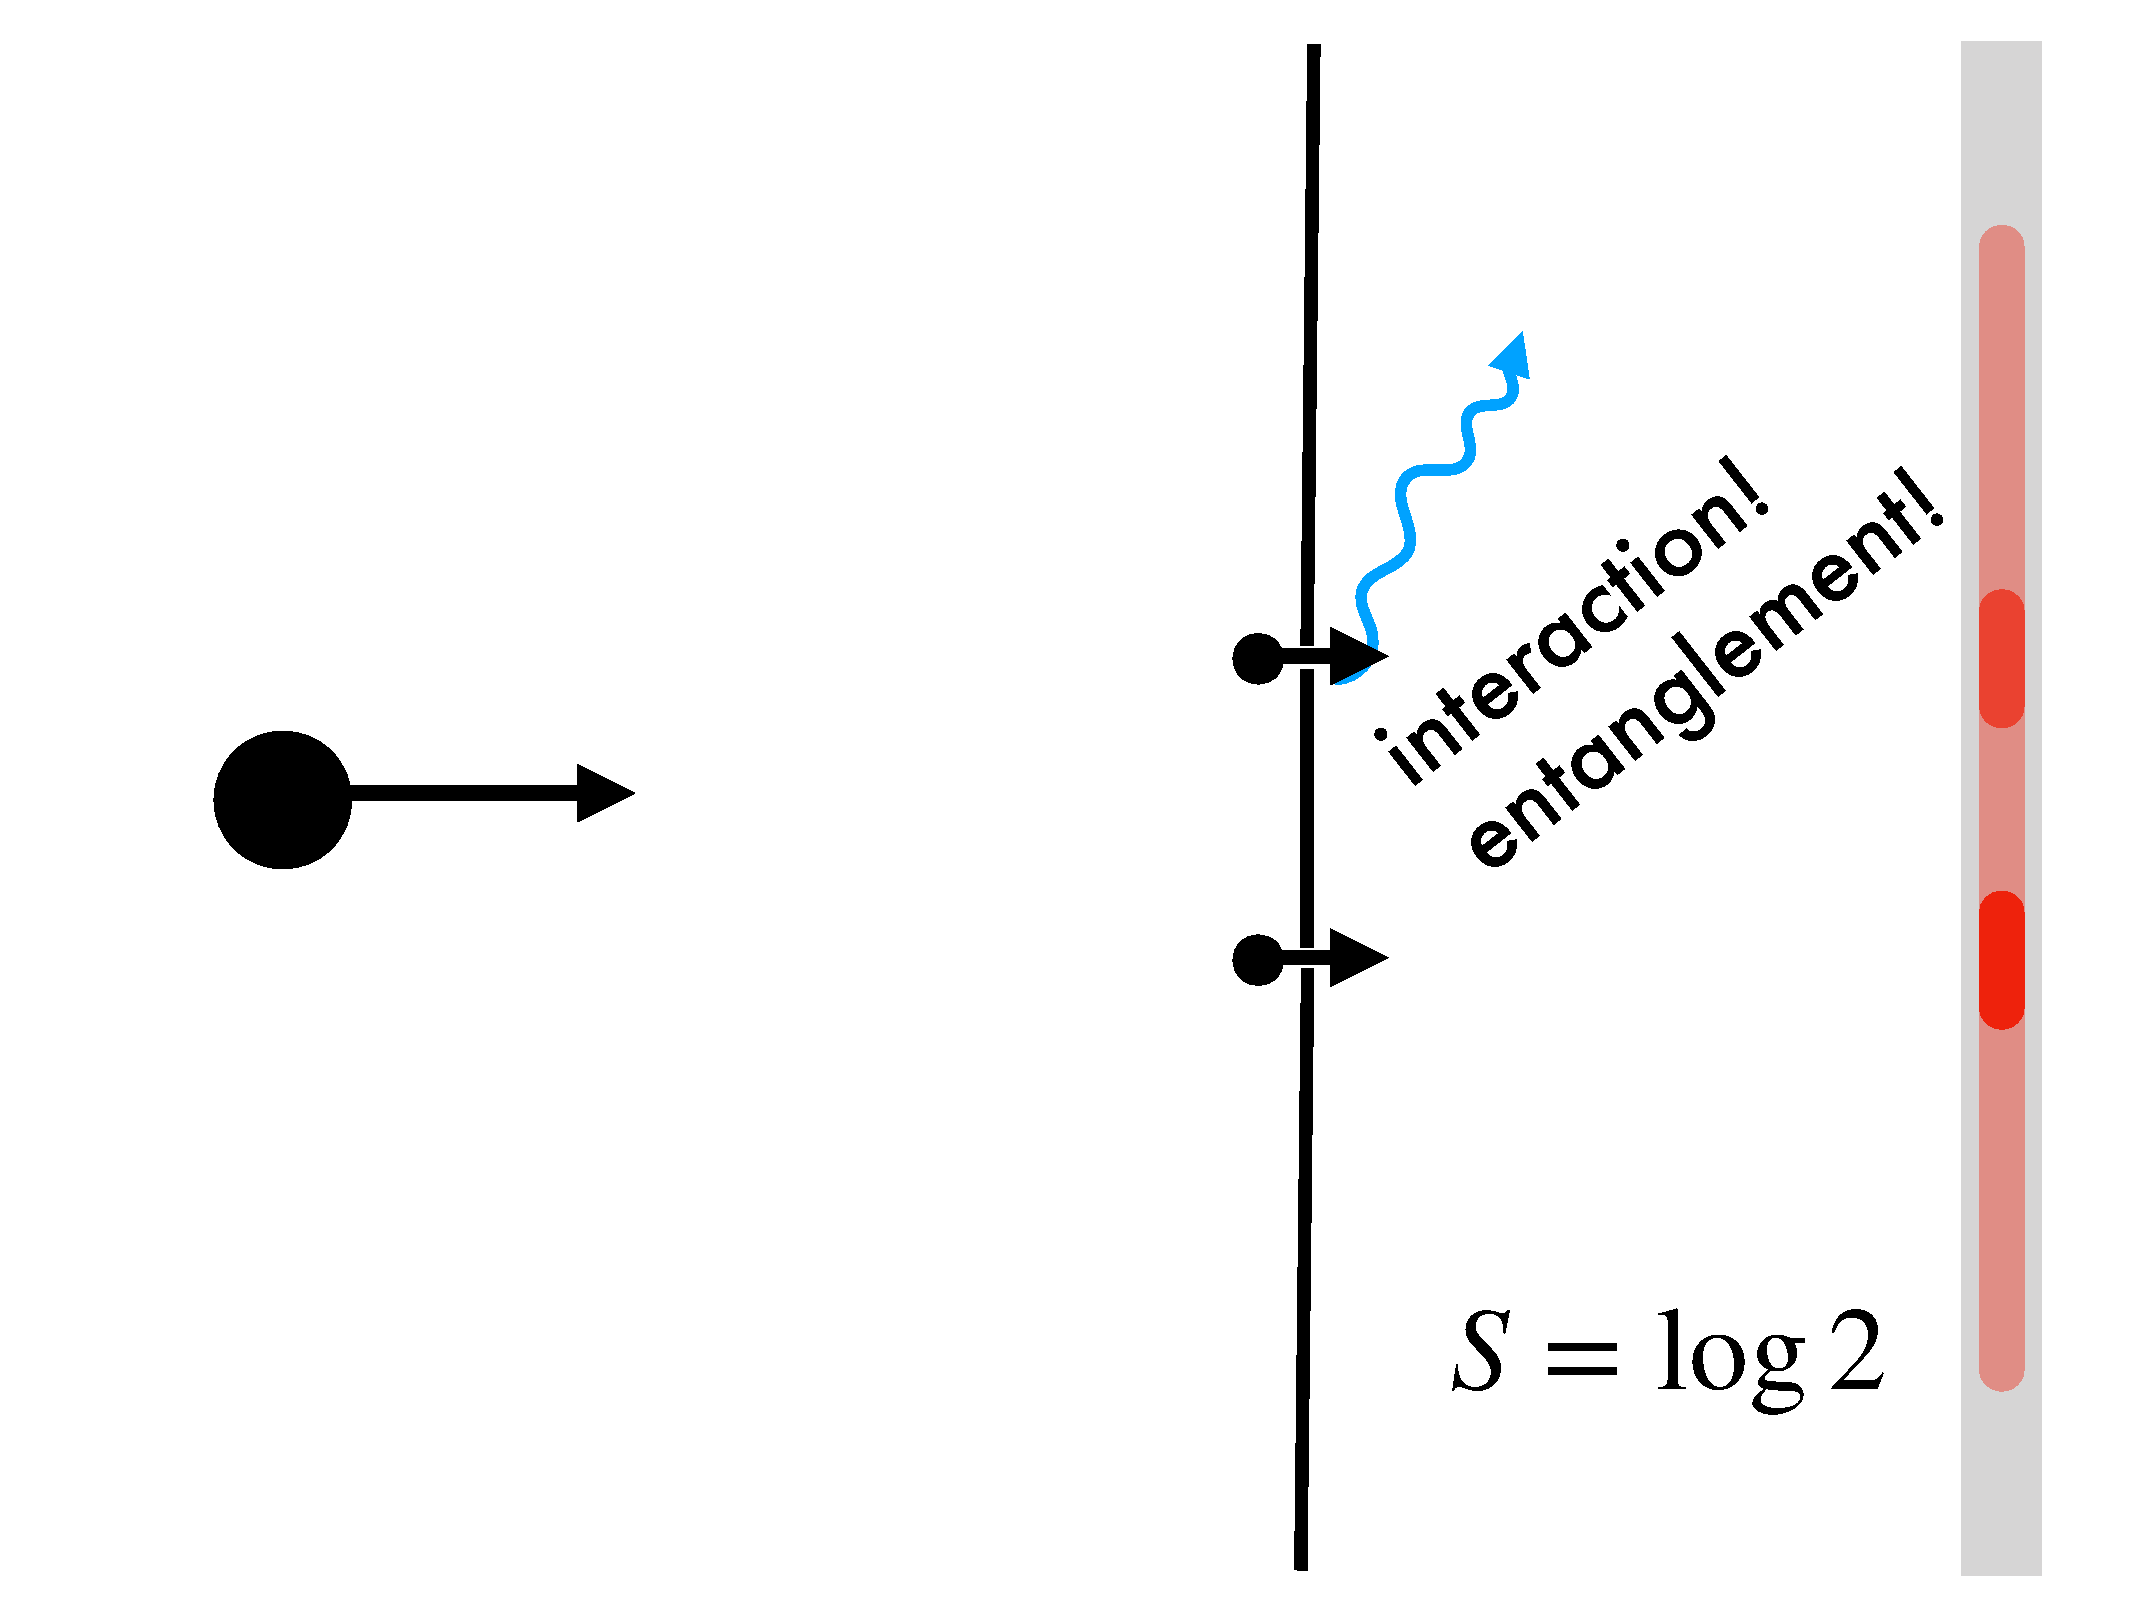
\includegraphics[width=\linewidth]{Figures/classical}
    \caption{Classical behaviour}
    \label{fig.classical}
    \end{framed}
\end{subfigure}
\caption{The double slit experiment.\label{fig.universeparts}}
\end{figure}

But what happens if we try to measure which slit the particle goes through, for example, by shooting photons at the location in the top slit? Then, we observe the fringe pattern predicted by classical mechanics, where the particle goes through only one slit (Figure \ref{fig.classical}). Let’s examine this process. To start, there is just the particle and the photons.
\[\ket{\text{particle}}\ket{\text{photons}}\]
If the particle doesn’t interact with the photons, it proceeds through the slits as before and does not become entangled with the photons.
\[\frac{1}{\sqrt{2}}\left(\ket{\text{through upper slit}} + \ket{\text{through lower slit}}\right)\ket{\text{photons}}\]
Because \(\braket{\text{through upper slit}}{\text{through lower slit}} \neq 0,\) we will have quantum interference and observe the result in Figure \ref{fig.quantum}. We calculate that the subsystem entropy for the particle is 0. 
On the other hand, if the part of the wavefunction in the upper slit becomes entangled with the photons, our state becomes
\[\frac{1}{\sqrt{2}}\left(\ket{\text{through upper slit}}\ket{\text{photons} \sim} + \ket{\text{through lower slit}}\ket{\text{photons}}\right)\]
where \(\ket{\text{photons} \sim}\)  is the state of the photons after the interaction. If \(\braket{\text{photons} \sim}{\text{photons}}=0\), then we will no longer have quantum interference. We will observe the result in Figure \ref{fig.classical}. The subsystem entropy of the particle is now \(\log 2\).

This process of losing quantum behaviour is called decoherence. Notice that the decoherence happened when the particle became entangled with the outside world.

In reality, some part of the wavefunction will interact while some will not. We will have some mix of the quantum and classical fringes. The entropy will be between \(0\) and \(\log 2\). It seems to quantify the amount of decoherence.

Finally, we note that the key property here was that \(\braket{\text{photons} \sim}{\text{photons}}=0\). If instead \(\braket{\text{photons} \sim}{\text{photons}}\neq0\), decoherence will not occur, though the subsystem entropy will still increase in the same way. Thus the subsystem entropy quantifies decoherence only if we assume that \(\braket{\text{photons} \sim}{\text{photons}}=0\).

\subsection{Decoherence is measurement by the universe}

Next I hope to dispel some of the magical aura (a.k.a. confusion) that surrounds how we should talk about decoherence as a concept. It is really quite simple: decoherence is measurement by the universe.

Physicists typically describe measurement as ``collapsing the wavefunction,’’ but what does this really mean? Suppose we start in a superposition of two possible outcomes.
\[
\frac{1}{\sqrt{2}}\left(\ket{\uparrow} + \ket{\downarrow}\right)\ket{\text{observer}}
\]
After a measurement, the observer has become entangled with the outcome.
\[
\frac{1}{\sqrt{2}}\left(\ket{\uparrow}\ket{\text{observed }\uparrow} + \ket{\downarrow}\ket{\text{observed }\downarrow}\right)
\]
Because \(\braket{\text{observed }\uparrow}{\text{observed }\downarrow}=0\), there is no more quantum interference between \(\ket{\uparrow}\) and \(\ket{\downarrow}\). To the observer, it looks as if the system has switched to either \(\ket{\uparrow}\) or \(\ket{\downarrow}\) (depending on which outcome was measured).

This process is exactly the same process as the decoherence that we saw in Section \ref{sec.doubleslit} It is exactly appropriate, therefore, to describe decoherence as ``the universe measuring the wavefunction.’’

(The description here is inspired by the confusingly-named ``many worlds interpretation'' of quantum mechanics, advanced by, for example, Sean Carroll \cite{Carroll}.)

\subsection{Entropy is entanglement with the universe}

We should note that whenever we talk about Von Neumann entropy, we are really talking about the Von Neumann entropy of a \emph{subsystem}. It doesn’t make sense to talk about the Von Neumann entropy of the \emph{whole universe} because there is just one possible wavefunction—the real one! We can only consider systems like the one in Figure \ref{fig.2part}. The subsystem entropy quantifies the amount of entanglement over the boundary between A and B. This, then, is what entropy is: a measure of how entangled a system is with ``everything else''.

``That’s fine,’’ another hasty physicist says, ``But what if you start in a classical superposition? You could start with more than one possible wavefunction for the whole universe simply because you don’t know which is correct. Then you have entropy without entanglement.’’ Saying this, the hasty physicist has made a mistake. He has forgotten that he is in the universe.

\begin{figure}[b]
\begin{subfigure}[t]{0.45\textwidth}
    \centering
    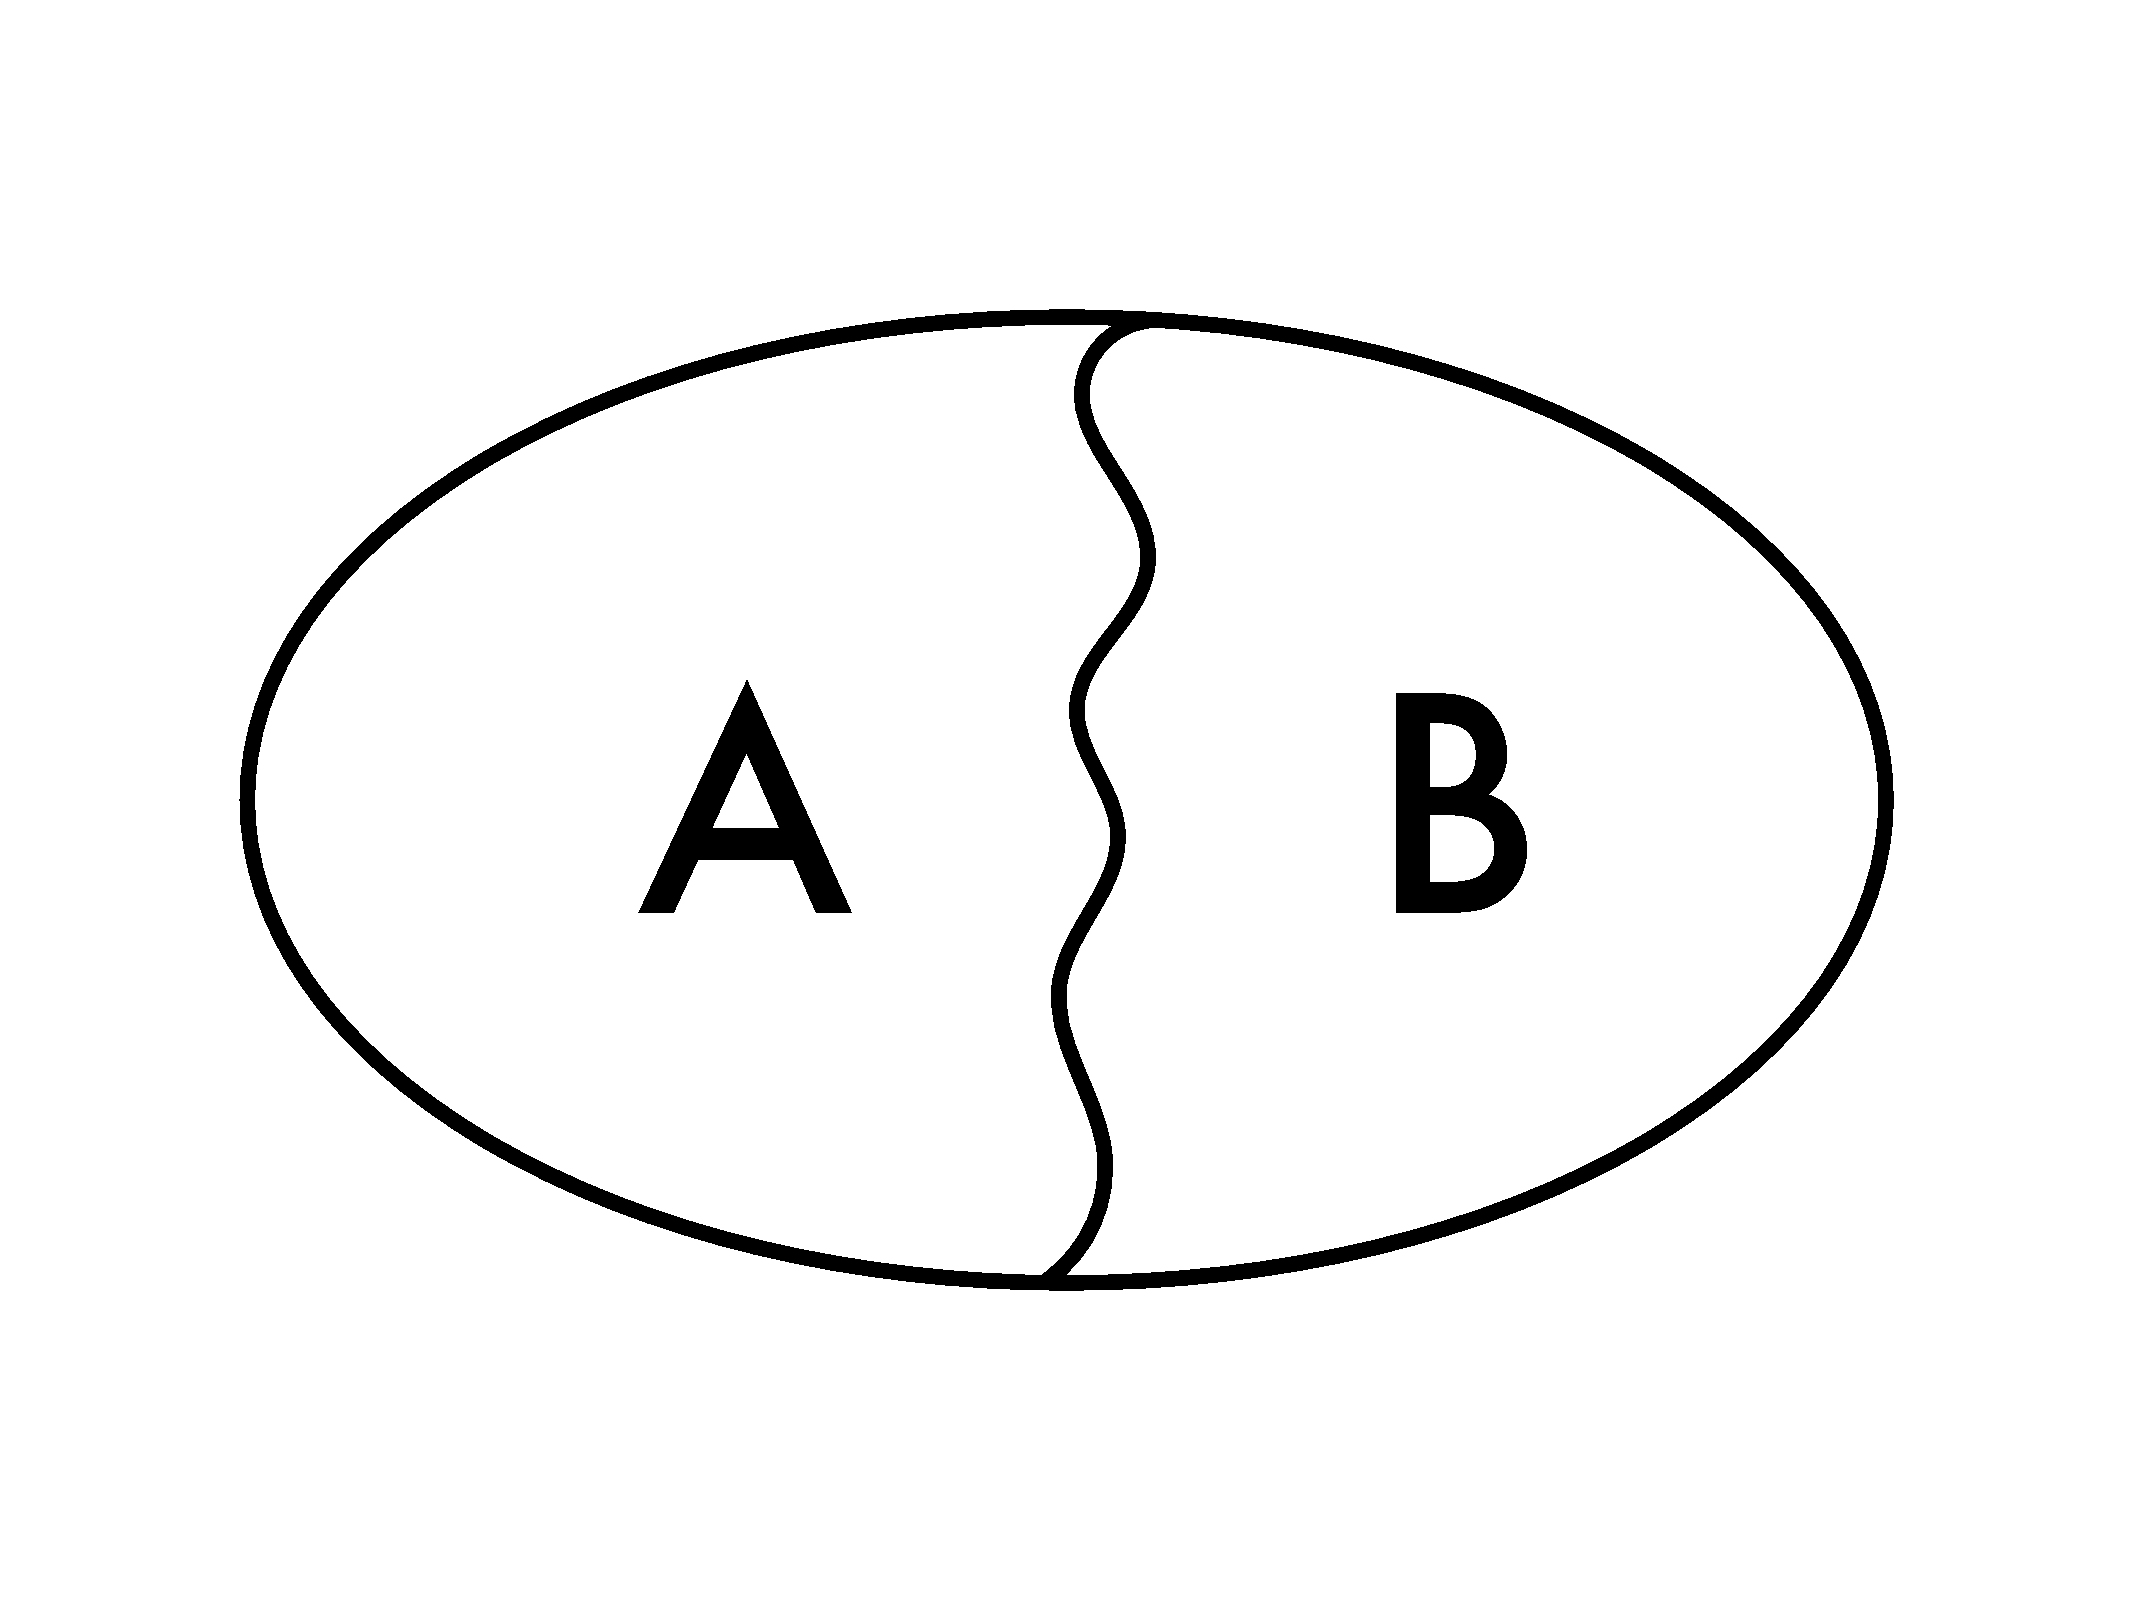
\includegraphics[width=\linewidth]{Figures/2part}
    \caption{Conceptualized}
    \label{fig.2part}
\end{subfigure}
\hfill
\begin{subfigure}[t]{0.45\textwidth}
    \centering
    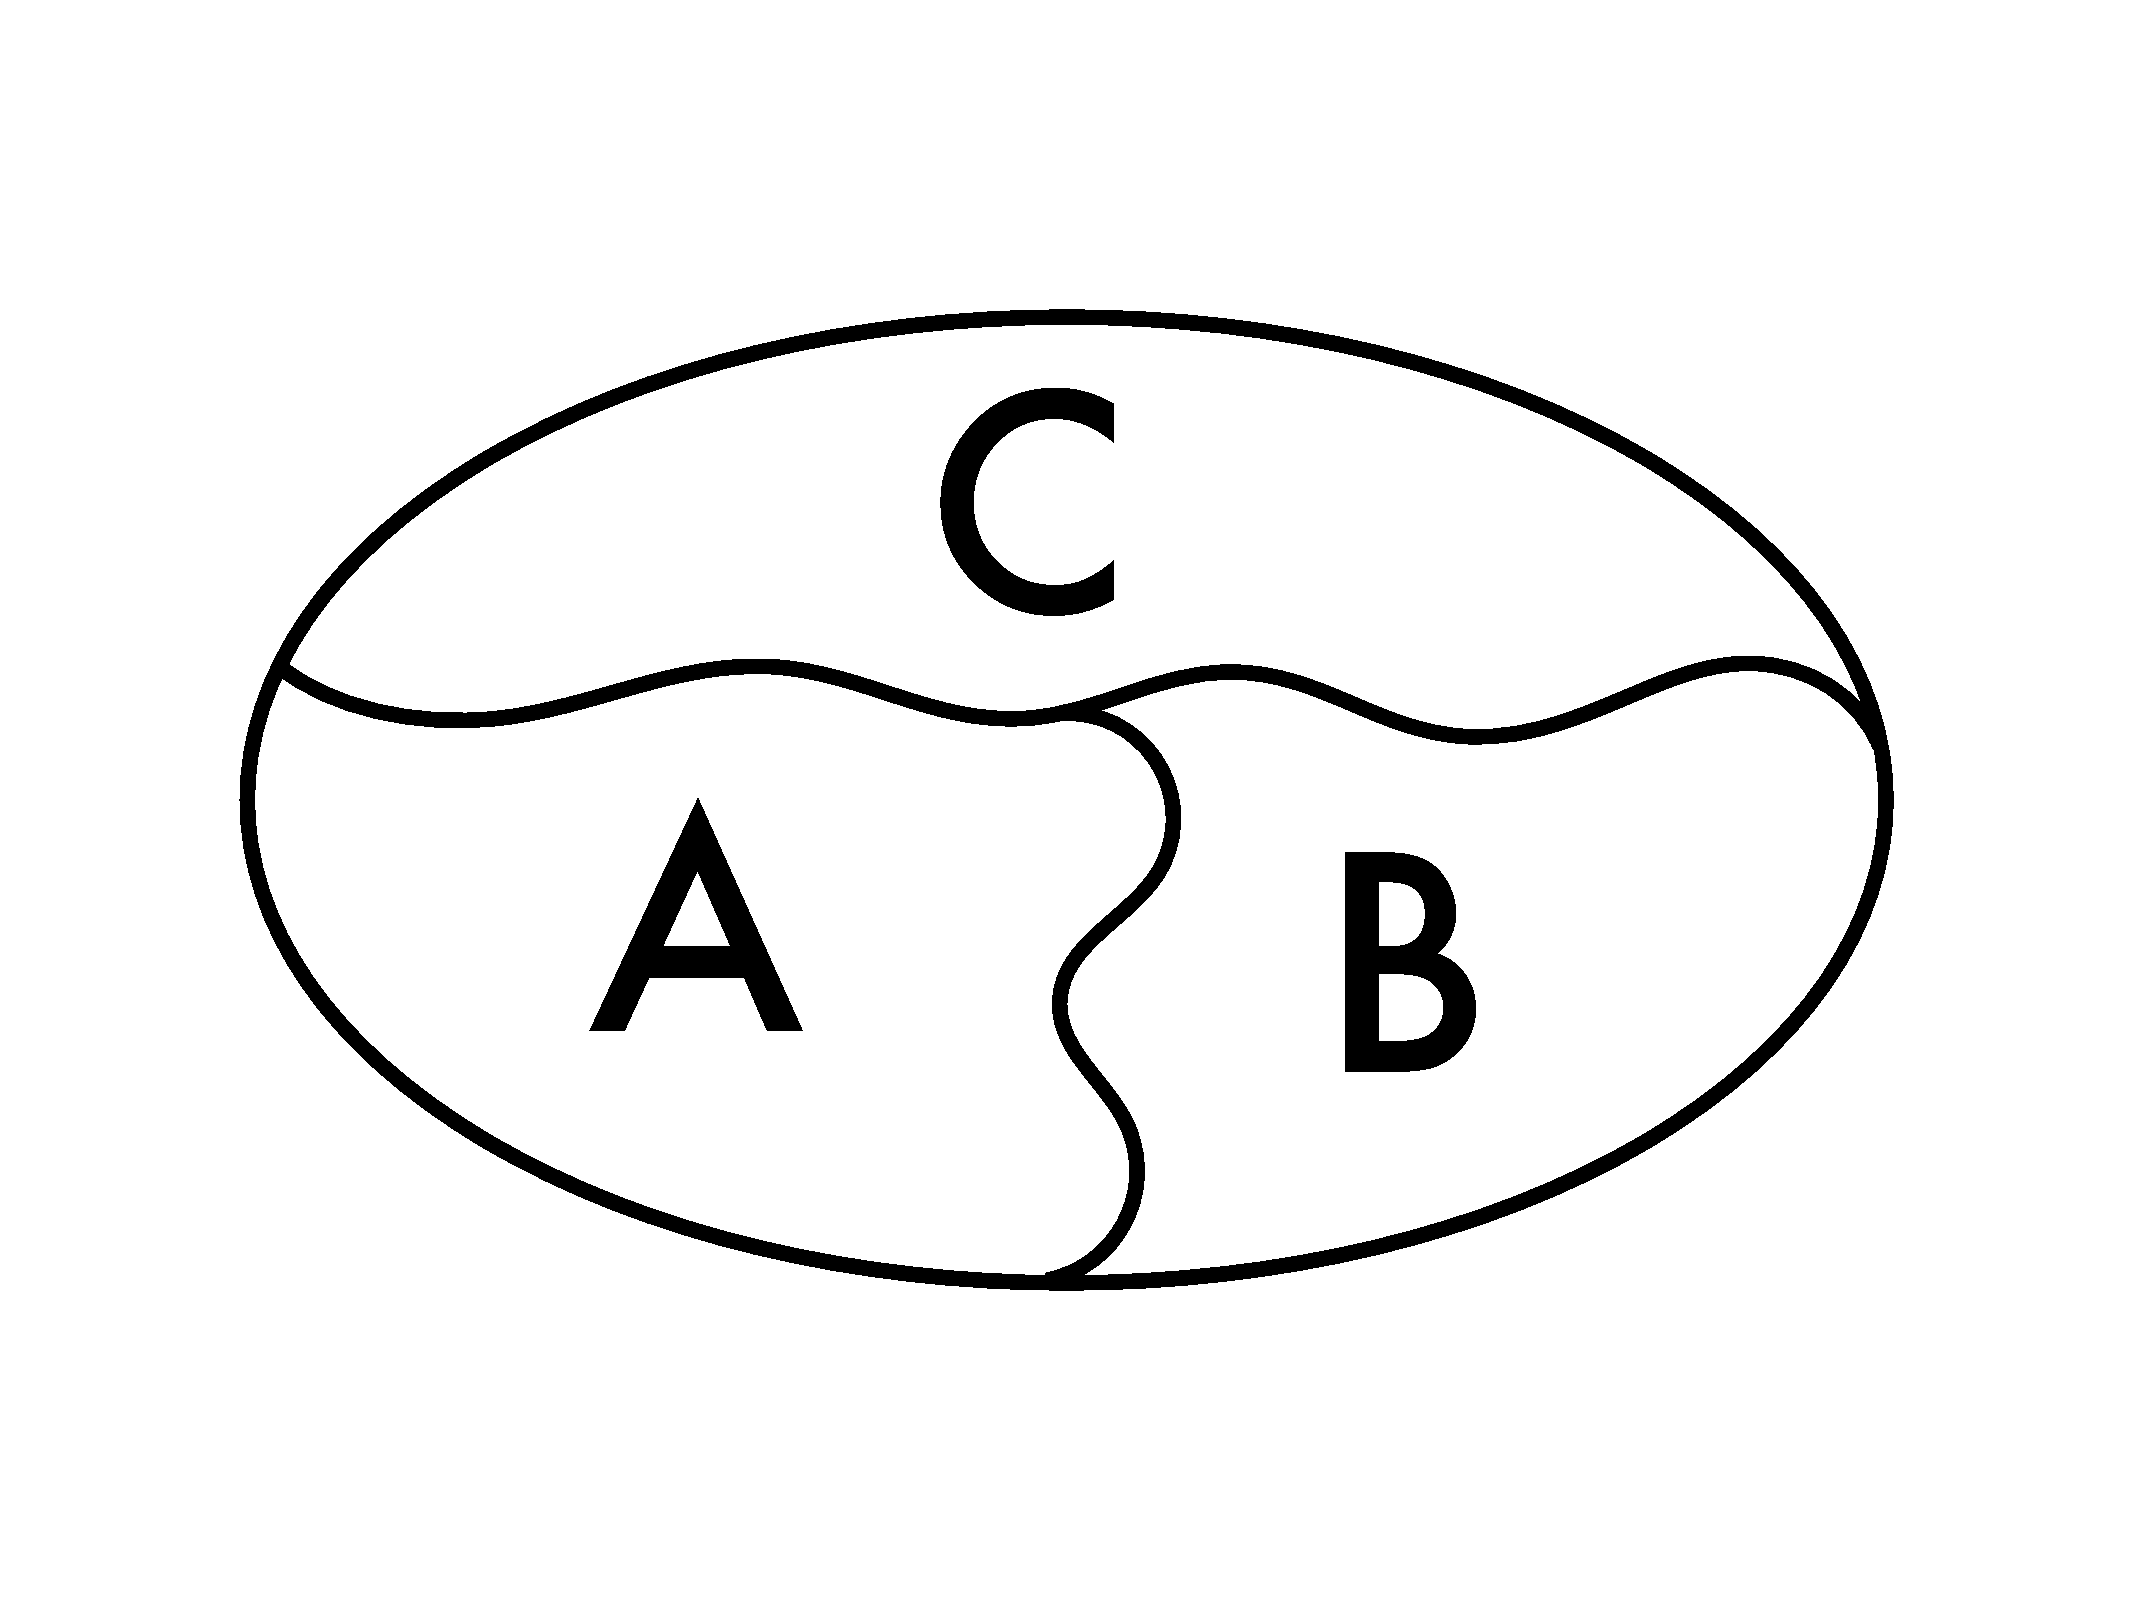
\includegraphics[width=\linewidth]{Figures/3part}
    \caption{Reality}
    \label{fig.3part}
\end{subfigure}
\caption{A bipartite system.}\label{fig.universeparts}
\end{figure}

The hasty physicist himself is already entangled with the system he wants to measure. Recall our messy room. The room’s owner has done things that cause a book to be here, a teapot to be there, and a pencil to be somewhere else, but he forgets what exactly he has done. Nevertheless his own state is entangled with the room’s state. If he had a perfect memory, the room would not seem messy, for he would know where everything is—but he has forgotten the nature of the entanglement. This fact does not alter that the entanglement exists.

The hasty physicist who says the A+B system can start in a classical superposition is really saying that there is a third part, C, that we ignore because it is impossibly complicated (Figure \ref{fig.3part}). When we say that A+B is in a classical superposition (mixed state), we really mean that A+B is entangled with C, but we already take the reduced density operator for the A+B system because we don’t know how to begin thinking about C. This does not alter that there is a single true global wavefunction for the universe. The hasty physicist has simplified life by averaging out the part of the universe he doesn’t understand. Having done so, when he computes the entropy of A, the hasty physicist is actually quantifying the entanglement of A with B \emph{as well as} the entanglement of A with C.

``Fair enough,’’ the hasty physicist says, ``But now you’re talking philosophy, not physics!’’ This interpretation, though, allows us to intuit \emph{physical} results by symmetries. Indeed, if we start with a pure state for A+B, that is, if A+B is truly unentangled with C, then the entropy of A and the entropy of B both quantify the entanglement across the A-B boundary. We expect both subsystems to have the same entropy. This is indeed what we find in Section \ref{sec.purestate}. Conversely, if A+B starts in a mixed state, that is, if A+B starts entangled with C, then the subsystem entropies of A and B will in general be different. The subsystem entropy of A includes entanglement across the A-C boundary, whereas the subsystem entropy of B includes entanglement across the B-C boundary, and these need not be equal. Again, this is what we find, in Section \ref{sec.separablestate}. (In Sections \ref{sec.separablestate} and \ref{sec.purestate}, I prove these conclusions only for diagonally separable states that can transition to new states in the accessible subspace. I conjecture that they can also be proven for other states. Future work should investigate this conjecture.)

While Figure \ref{fig.3part} is the correct picture, it is still useful for computational purposes to pretend that C doesn’t exist (as the hasty physicist thinks). We need not complicate our derivations by acknowledging it.

Note that entropy measures entanglement with the universe, which is not the same thing as \emph{decoherence}. Decoherence requires that the states the system is entangled with are orthogonal in the universe’s space. In practice, however, it is often reasonable to assume that they are orthogonal. This is why it makes sense to describe entropy as quantifying decoherence.

Of course, it is somewhat arbitrary where one draws the boundaries between A, B, and C. Taking the perspective of the whole universe, there is just a wavefunction. We conjure up mixed states due to our imperfect understanding. 
Henry Adams wrote, “Chaos was the law of nature; order was the dream of man.” Perhaps we may now say instead, rather more optimistically, “Order is the law of nature; chaos is the dream of man.”

